% Schema of Labs on a class
% Author: Cristo J. Alanis
\documentclass[11pt]{article}
\usepackage{tikz}
\usetikzlibrary{shadows,arrows}
% Define the layers to draw the diagram
\pgfdeclarelayer{background}
\pgfdeclarelayer{foreground}
\pgfsetlayers{background,main,foreground}

% Define block styles  
\tikzstyle{block}=[draw, fill=blue!20, text width=7.0em, text centered,
minimum height=1.5em,drop shadow]
\tikzstyle{blocks} = [block, rounded corners, drop shadow]
\tikzstyle{texto} = [above, text width=6em, text centered]
\tikzstyle{linepart} = [draw, thick, color=black!50, -latex', dashed]
\tikzstyle{line} = [draw, thick, color=black!50, -latex']
\tikzstyle{ur}=[draw, text centered, minimum height=0.01em]

% Define distances for bordering
\newcommand{\blockdist}{1.3}
\newcommand{\edgedist}{1.5}

\newcommand{\external}[2]{node (e#1) [blocks]
	{External 12V Supply\\{\scriptsize\textit{#2}}}}

\newcommand{\regulator}[2]{node (r#1) [blocks]
	{Voltage Regulation\\{\scriptsize\textit{#2}}}}

\newcommand{\uC}[2]{node (uC#1) [blocks]
	{$\mu$Controller\\{\scriptsize\textit{#2}}}}

\newcommand{\uart}[2]{node (uart#1) [blocks]
	{PC UART Interface\\{\scriptsize\textit{#2}}}}

\newcommand{\prog}[2]{node (prog#1) [blocks]
	{Programming / Debug Interface\\{\scriptsize\textit{#2}}}}

\newcommand{\motor}[2]{node (motor#1) [blocks]
	{Motor\\{\scriptsize\textit{#2}}}}

\newcommand{\sigcond}[2]{node (sigcond#1) [blocks]
	{Signal Conditioning\\{\scriptsize\textit{#2}}}}

\newcommand{\encdig}[2]{node (encdig#1) [blocks]
	{Digital Logic Circuit\\{\scriptsize\textit{#2}}}}

\newcommand{\pc}[2]{node (pc#1) [blocks]
	{PC\\{\scriptsize\textit{#2}}}}

\newcommand{\physical}[2]{node (physical#1) [blocks]
	{Physical Model\\{\scriptsize\textit{#2}}}}

\newcommand{\motordriver}[2]{node (motordriver#1) [blocks]
	{Motor Driver\\{\scriptsize\textit{#2}}}}

\newcommand{\digitlogic}[2]{node (digitlogic#1) [blocks]
	{Digital Logic Circuit\\{\scriptsize\textit{#2}}}}

\newcommand{\encoder}[2]{node (encoder#1) [blocks]
	{Hall Effect Encoder\\{\scriptsize\textit{#2}}}}
% Draw background
\newcommand{\background}[5]{%
	\begin{pgfonlayer}{background}
		% Left-top corner of the background rectangle
		\path (#1.west |- #2.north)+(-0.5,0.5) node (a1) {};
		% Right-bottom corner of the background rectanle
		\path (#3.east |- #4.south)+(+0.5,-0.25) node (a2) {};
		% Draw the background
		\path[fill=yellow!20,rounded corners, draw=black!50, dashed]
		(a1) rectangle (a2);
		\path (a1.east |- a1.south)+(0.8,-0.3) node (u1)[texto]
		{\scriptsize\textit{Unidad #5}};
\end{pgfonlayer}}

\newcommand{\transreceptor}[3]{%
	\path [linepart] (#1.east) -- node [above]
	{\scriptsize Transreceptor #2} (#3);}

\begin{document}
	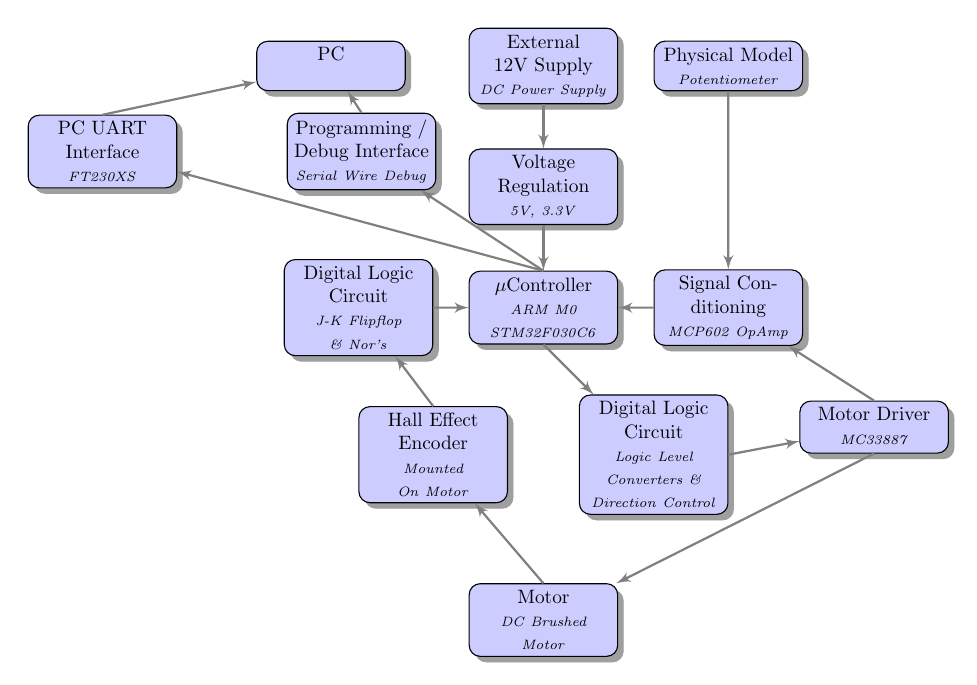
\begin{tikzpicture}[scale=0.7,transform shape]
	
	% Draw diagram elements
	\path \external {1}{DC Power Supply};
	\path (e1.east)+(2.0,0.0) \physical{1}{Potentiometer};
	\path (e1.south)+(0.0,-1.5) \regulator{1}{5V, 3.3V};
	\path (r1.south)+(0.0,-1.5) \uC{1}{ARM M0 STM32F030C6};
	\path (uC1.south)+(-8,3.5) \uart{1}{FT230XS};
	\path (uC1.south)+(-3.3,3.5) \prog{1}{Serial Wire Debug};
	%\path (uC1.east)+(2.0,0) \dirlogic{1}{};
	\path (uC1.east)+(2.0,0) \sigcond{1}{MCP602 OpAmp};
	\path (uC1.west)+(-2.0,0) \encdig{1}{J-K Flipflop \& Nor's};
	\path (uC1.south)+(6,-1.5) \motordriver{1}{MC33887};
	\path (uC1.south) + (0,-5) \motor{1}{DC Brushed Motor};
	\path (uC1.south) + (2,-2) \digitlogic{1}{Logic Level Converters \&  Direction Control};
	\path (uC1.south)+ (-2,-2) \encoder{1}{Mounted On Motor};
	
	\path (e1.west)+(-2.5,0) \pc{1}{};
	
	
	% Draw arrows between elements
	\path [line] (e1.south) -- node [above] {} (r1);
	\path [line] (r1.south) -- node [above] {} (uC1);
	\path [line] (uC1.north) -- node [above] {} (uart1);
	
	\path [line] (uC1.north) --node [above]{}(prog1); 
	\path [line] (encdig1.east) --node [left]{}(uC1);
	\path [line] (sigcond1.west) -- node[right]{}(uC1);
	\path [line] (physical1.south) -- node[above]{}(sigcond1);
	\path [line] (motordriver1.north) -- node[below]{}(sigcond1);
	\path [line] (uart1.north) -- node[below]{}(pc1);
	\path [line] (prog1.north) -- node[below]{}(pc1);
	\path [line] (motordriver1.south) -- node[above]{}(motor1); 
	\path [line] (uC1.south) -- node[above]{}(digitlogic1);
	\path [line] (digitlogic1.east) -- node[left]{}(motordriver1);
	\path [line] (encoder1.north) -- node[below]{}(encdig1);
	\path [line] (motor1.north) -- node[below]{}(encoder1);
	\end{tikzpicture}
\end{document} 